%
% You may wish to use some of the following options of the iitthesis
% package:
%
% fullpageDraft      avoid the margins necessary for proper binding and
%   just view or print a draft.
% beforeDefense      makes the personal acknowledgements invisible;
%   use this to print the copies you submit initially to the grad school
%   for sending to the opponent panel, i.e. thesis readers (who shouldn't
%   see those parts). For the final submission, after having successfully
%   defended - drop this option.
% noabbrevs          no notation & abbreviations list will be included
%   in the thesis.
%
% Additionally, you must specify the degree for which you're writing
% your thesis (MSc/PhD/MArch etc.)
%
\documentclass[PhD,noabbrevs]{misc/iitthesis}


% Definitions of info fields for the thesis - subject, advisor,
% faculty, acknowledgements, etc. etc. This file must contain Hebrew
% text, so the question of its character set encoding is significant.
% This templated uses the iso-8859-8-i charset (i.e. single-byte logical 
% Hebrew; it's about the same as the windows-1255 codepage, but not the
% same as UTF-8) - and this works with MikTeX 2.9 and using pdfelatex.
% With your TeX distribution you might need to create files in the
% UTF-8 charset.
% This file contains definitions of various fields used
% in various places throughout the thesis (in the title
% pages mostly). Whatever isn't define here has some
% default (and usually irrelevant) text.

%\authorEnglish{Mish Talem}
%\authorHebrew{מש תלם}

%\titleEnglish{Improved methods \\ for the cultivation of lettuce \\ on the coastal plane}
%\titleHebrew{שיטות משופרות \\ לגידול חסה במישור החוף}

\disciplineEnglish{Computer Science}
\disciplineHebrew{מדעי המחשב}

\supervisionEnglish{This research was carried out under the supervision of Prof.~Big Shot, in the Faculty of Computer Science.}
\supervisionHebrew{המחקר בוצע בהנחייתו של פרופסור אישחשוב עצמוני, בפקולטה למדעי המחשב.}

\GregorianDateEnglish{January 2012}
\GregorianDateHebrew{ינואר \textenglish{2012}}
\JewishDateEnglish{Tevet 5772}
\JewishDateHebrew{טבת התשע"ב}

%\financialAcknowledgementEnglish{The Technion's funding of this research is hereby acknowledged.}
%\financialAcknowledgementHebrew{הכרת תודה מסורה לטכניון על מימון מחקר זה.}

\publicationInfoEnglish{%
%Remove this parenthesized note and the line following it!
(The grad school guidelines now require that you mention the following regarding publications of your thesis work; but of course, remove this parenthesized note...; you will find the note in the \texttt{thesis-fields.tex} file. The entries for the publication list are BiBTeX bibliography entries, separate from those in the main bibliography: You must place them in \texttt{front/pubinfo.bib}; make sure their labels are distinct from entries in the main bibliography; and order them in the order in which you want them to appear --- they will not be sorted. Note also that the document may need to be processed several times before the list of publications actually appears)

Some results in this thesis have been published as articles by the author and research collaborators in conferences and journals during the course of the author's doctoral research period, the most up-to-date versions of which being:

\butcheredbibliography{pubinfo}{front/pubinfo}
}

\publicationInfoHebrew{%
(התייחסות לפרסומים, שמופיעה להלן, הינה הכרחית לפי תקנות ביה"ס ללימודי מוסמכים; כמובן שיש למחוק את ההערה הזו שבסוגריים... תוכן זה נמצאה בקובץ \textenglish{\texttt{thesis-fields.tex}}. הרשומות לצורך רשימת הפרסומים הינן רשומות \textenglish{BibTeX}, נפרדות מן הרשומות בביבליוגרפיה העיקרית של המסמך: עליך לשים אותן בקובץ \textenglish{\texttt{front/pubinfo.bib}}; הקפיד/י שהתוויות שלהם יהיו שונות מתוויות הרשומות בביליוגרפיה העיקרית. רשום/י אותם בסדר בהם תרצה/י שיופיעו ברשימה --- שכן הן לא ימוינו. כן שים/י לב שייתכן שיהיה צורך להדר את המסמך פעם או פעמיים נוספות עד שהרשימה אכן תופיע כראוי.)

חלק מן התוצאות בחיבור זה פורסמו כמאמרים מאת המחבר ושותפיו למחקר בכנסים ובכתבי-עת במהלך תקופת מחקר הדוקטורט של המחבר, אשר גרסאותיהם העדכניות ביותר הינן:%

\begin{otherlanguage}{english}%
% No need to mention the bibliography file this time, as it has already been used in
% the English invocation
\butcheredbibliography{pubinfo}{front/pubinfo}
\end{otherlanguage}%
}

\thesisbibfiles{back/general}
\thesisbibstyle{alpha}


% Personal acknowledgements (are only used for the post-exam
% version)
\personalAcknowledgementEnglish{
I would like to thank my advisor, my parents, my friends, etc. etc.

Add any thank-yous, acknowledgements, personal comments you wish to make here (in \texttt{personal-acks.tex}).

Note that this acknowledgements section only gets printed in the post-exam version of the thesis (i.e. if you leave out the \texttt{beforeExam} package option.)
}

\personalAcknowledgementHebrew{

אני רוצה להודות למנחה שלי, להוריי, לחבריי, וכו' וכו'.

אפשר להוסיף עוד תודות והערות אישיות כאן.

שים/י לב: קטע זה של תודות מודפס בפועל רק בגרסת החיבור שלאחר-הבחינה
 (הווה אומר רק אם הסרת את האפשרות
\texttt{beforeExam}
 מאפשרויות החבילה.)
}


% The abstract in Hebrew and in English should have its own file.
%
% Notes:
% - You can split this one, and have separate files for the English
%   and the Hebrew abstract
% - regulations require the English abstract contain between 200 and
%   500 words, and the Hebrew abstract contain between 1,000 and 2,000
%   words (making it something between an abstract and an introduction
%   with an overview of results).
% - Be careful with links in Hebrew text (wrap them in \L{}).
% Just write down your abstract here, no special commands necessary except for the \abstractEnglish{
% before this text is used and a closing } at the end of it

\abstractEnglish{

At this point you write the abstract of your work, in the main language in which it is written (in this template - English). Graduate school regulations require the abstract to constitute an independent whole and be understood to a reader with general knowledge of the field. Use complete sentences and make few or no citations. Do not refer to the main body of the work and do not use uncommon shorthand, symbols and terms unless you have room for explaining them. The English abstract should be between 200 and 500 words long.

So this should contain a few more paragraphs...

\lipsum[10-12]

}

% Note that various commands don't work that well in Hebrew. Specifically,
% if you're using hyperref, you'll have trouble with \url, \autoref, \cite
% and friends. iitthesis-extra.sty has a workaround: the \disabledlinksL
% command. See the .sty for details, or:
% http://tex.stackexchange.com/q/32466/5640 for

\abstractHebrew{

כאן יבוא תקציר מורחב בעברית (כאשר שפת החיבור העיקרית היא אנגלית). היקף התקציר יהיה \textenglish{1000-2000} מילים. התקציר יהווה שלמות בפני עצמו ויהיה מובן לקורא בעל ידיעות כלליות בנושא.

בית הספר ללימודי מוסמכים מנחה מספר הנחיות לגבי התקציר בעברית:
\begin{itemize}
\item על התקציר להיכתב במשפטים מקושרים שלמים.
\item בדרך-כלל אין לציין בתקציר מקורות ספרותיים וציטוטים.
\item אין להתייחס למספר של פרק, סעיף, נוסחה, ציור או טבלה שבגוף החיבור, ואין להשתמש בקיצורים, סמלים ומונחים לא מקובלים, אלא אם יש בתקציר די מקום לזיהויים.
\end{itemize}

לעתים יש בכל-זאת יש צורך לכלול פקודה הכוללת קישור פנימי או חיצוני בתוך התקציר העברי; במצבים כאלו כדאי דרך-כלל לעטוף את הפקודה היוצרת את הקישור בתוך פקודת \textenglish{\texttt{\textbackslash{}textenglish\{\}}} כדי למנוע כל מיני פורענויות בלתי-רצויות, כגון כישלון בהידור קובץ ה-\textenglish{PDF} או שימוש בגופן העברי באופן אשר עלול שלא להנעים לעין. לדוגמה: נניח שיש לנו צורך לצטט מקור ביבליוגרפי. אם נעשה זאת סתם-כך: \textenglish{\texttt{\textbackslash{}cite\{Hoeffding\}}}, נקבל: \cite{Hoeffding}; אם נעטוף את פקודת הציטוט, כך: \textenglish{\texttt{\textbackslash{}textenglish\{\textbackslash{}cite\{Hoeffding\}\}}}, נקבל \textenglish{\cite{Hoeffding}} (כפי שהציטוטים נראים גם בטקסט באנגלית).

\subsection*{\texthebrew{תת-חלק בתקציר המורחב}}

תוכן מקוצר לגבי נושא מסוים. התייחסות ל\emph{מושג} מסוים שהחיבור בוחן. וכולי וכולי.


\subsection*{\texthebrew{נקודה מעניינת לגבי העמודים בעברית}}

שימו לב כי העמודים בעברית אמורים להיות מיוצרים בסדר ה''הפוך'', הווה אומר העמוד האחרון בקובץ ה-\textenglish{PDF} הוא הכריכה העברית, לפניו השער העברי, ודפי התקציר צריכים להופיע בסדר הפוך (וכן במספור רומי, לפי נהלי הטכניון). כך אם נתבונן במספר שבתחתית עמוד זה \textenglish{---} אשר צריך להיות העמוד הראשון בתקציר-המורחב מבחינת רצף התוכן, והינו העמוד האחרון מבין עמודי התקציר-המורחב אחרון בקובץ ה-\textenglish{PDF} \textenglish{---} נמצא את המספר \textenglish{i} ...

\newpage

... ואילו עמוד זה של התקציר-המורחב בעברית \textenglish{---} שהינו העמוד השני בתקציר-המורחב מבחינת רצף התוכן, ונמצא ראשון בקובץ ה-\textenglish{PDF} \textenglish{---} ממוספר ב-\textenglish{ii}. המטרה במספור בסדר ה"הפוך" היא, שבעת ההדפסה לא יהיה צורך להפוך דפים, לשנות את סדרם וכולי \textenglish{---} רק להדפיס ולכרוך.

}

% Use this file to create "glossary entries" for abbreviations and acronyms.
% The entries defined here don't necessarily have to be used in the thesis.

\newacronym[%
    description=``The Senate and People of Rome'']%
    {spqr}{SPQR}{Senātus Populusque Rōmānus}

\newacronym[%
    description=``A technology used in data storage devices'']%
    {smart}{SMART}{Self-Monitoring, Analysis and Reporting Technology}

\newglossaryentry{symb:c}{%
  name=$c$,%
  description=the speed of light%
}

\newglossaryentry{symb:a-b}{%
  name=\ensuremath{a \pm b},%
  description=the closed interval \ensuremath{\left[a-b,a+b\right]}%
}

\newglossaryentry{supercali}{%
  name=supercalifragilisticexpialidocious,
  description=%
    Atoning for being educable through delicate beauty.
    Something to say when you have nothing to say.}

% --------------------------------

% Commands below will control the behavior/appearance of the list of abbreviations and acronyms

% Print long form of acronym first with short in parenthesis
\setabbreviationstyle[acronym]{long-short}


% Uncomment this command to have _all_ abbreviations and acronyms defined
% in this file appear in the final list - rather than just the ones you
% use in the thesis
%\keepUnusedAbbreviations


% Additional machinery relevant to any thesis
% (it's not part of the document class because it's not absolutely
% necessary and not everyone might like it)
\usepackage{misc/iitthesis-extra}

% Definitions useful for anything you write, which you also
% include in any articles, presentations, HW assignments and other
% documents. May contains macros for notation algebra, logic,
% calculus and other fields, as well as general shorthands and
% LaTeX tricks, and package use commands
% General-purpose definitions and inclusions
% you are using in any document 
% (regardless of its class and style files used),
% e.g. package uses:

%\usepackage{xspace}

% and macros/command defintions:

%\newcommand{\complexityclass}[1]{{\bf #1}\xspace}
%\newcommand{\NPTIME}{\complexityclass{NP}}

% For this template, we'll only have one single command,
% necessary for including graphics...
\usepackage{graphicx}% http://ctan.org/pkg/graphicx


% Definitions, settings and tweaks for this thesis specifically

% This file should contain your own definitions specific
% only to this thesis;

% What it contains below is used 
% simply for generating dummy text in the sample 
% content provided with the template (see mainchap1.tex);
% so you can safely delete this when creating your own
% thesis

\usepackage{lipsum}
% ... needs a workaround for babel compatibility, see:
% http://tex.stackexchange.com/q/49214/5640
\makeatletter
\renewcommand\lips@dolipsum{%
  \ifnum\value{lips@count}<\lips@max\relax
    \addtocounter{lips@count}{1}%
    \csname lipsum@\romannumeral\c@lips@count\endcsname
    \lips@dolipsum
  \fi
}
\makeatother

% Another dummy text generator...
\def\qbfox#1{%
  \count1=0%
  \loop%
    \ifnum\count1<#1%
      \advance\count1 by 1%
      The quick brown fox jumped over the lazy dog. %
      \repeat%
  \relax%
}



% If you are using WinEdt, and using a publication list on the the
% acknowledgements page, and are having problems getting your document
% to compile with the 'PDFLaTeXify' button, try uncommenting the
% following two lines;
% Also, you will need to PDFLaTeXify at least twice, as WinEdt misses
% an extra run. See also:
% http://tex.stackexchange.com/q/41727/5640
\usepackage{multibib}
\newcites{pubinfo}{Acknowledgement page references}
\def\iitthesisextramultibibdefs{}

\begin{document}

% Front Matter
% ------------

% The following command will typeset the outer cover page, the
% inner title page, the acknowledgements page, etc. - everything
% up to but not including the introduction
\makefrontmatter

% Main Matter
% ------------
%
% To conform to Technion regulations, the main matter should begin
% with an introduction (including a survey of relevant past work):
%


\chapter{Introduction}
\label{chap:intro}
% do we need to add TOC lines?

%\begin{figure}
%  \centering
%  \includegraphics[width=0.75\textwidth]{main/graphics/a_blowup.pdf}
%  \caption{This is a caption}
%\end{figure}

Here you can introduce the field, survey past results, give context, use citations of course... (e.g. \cite{Papadimitriou1994}). It is probably worthwhile to clarify the goals or targets of the research and describe the process, unless this is done later.

You can also introduce \emph{a key concept} (or rather, several) without formally defining them until later on.

\subsection*{An unnumbered subsection}

You may want to break up the intro into parts with titles. Subsectioning without numbering is an option you might want to consider.

Some people include a specific section overviewing the results ("In Chapter so-and-so, we will see how etc.") which is also a way of describing the structure of the thesis. But this is not necessary.

\subsection*{Thesis options and appearance}

Please note that the \texttt{iitthesis} class has several options when you use it, such as:
\begin{itemize}
\item \texttt{fullpageDraft} to avoid the margins necessary for proper binding when you make the final print
\item \texttt{beforeExam} makes the personal acknowledgements invisible; use this to print the copies you submit initially to the grad school for sending to the examiners (who shouldn't see these). For the final submission, drop this option.
\item \texttt{noabbrevs} no notation \& abbreviations list will be included in the thesis.
\end{itemize}


%
% and then cover:
% - The methods used in the research
% - The research results
% - Discussion and conclusions from the results
%
% but not necessarily with a specific chapter for each of them.
%
% Then you have your main chapters (although these might still
% include an initial chapter on technical preliminaries, experimental
% system setup, and/or a final chapter with summary, discussion and further
% research direction or questions)


\chapter{Preliminaries}
\label{chap:prelims}

A preliminaries chapter is not necessary, but it may be a good idea to use it for presenting your theoretical/mathematical framework in a more detailed and technical way than the introduction, and to perhaps establish some basic lemmata/observations common to multiple chapters of your thesis.

\section{Some section}

Let's define some concept we'll be using throughout the thesis.

\begin{definition}
The \emph{von Neumann model} of a computer, also known as the \emph{Princeton architecture} is an architecture for digital computers, which consists of a processing units, containing an ALU and processing registers; a control unit consisting of an instruction register and a program counter; a memory unit which stores both data and instructions; and input-and-output mechanisms.
\end{definition}


\chapter{A main chapter}
\label{chap:firstchap}

\section{Introduction}

You might have a per-chapter mini-intro, possibly tying in to the relevant part of the general intro.

\section{A section}

\lipsum[1]

Let's cite a source: \cite{Yao1977}. And now,  let's introduce a (numbered) equation...
\begin{align}
\label{eq:emc2}
e &= mc^2
\end{align}

\begin{note}
	Are you seeing a problem with the equation numbering? In some TeX processors and on some platforms, there may be a layout error, so that instead of ``(3.1)'' you get ``)3.1)'' or some other flipping of directions. Specifically, \url{http://overleaf.com} suffers from this problem (at least until 2020). Please make sure and use an appropriate TeX distribution that's up-to-date. Specifically, recent TeXLive versions work fine. On Overleaf, you can switch TeXLive versions using the main menu.
\end{note}

In \autoref{sec:thm-like} below, we will state some theorems.

\section{Results... and theorem-like environments}
\label{sec:thm-like}

What's so special about the theorem-like environments used here? There are several packages which offer the capability of defining these, mainly \texttt{amsthm}, \texttt{ntheorem} and also \texttt{thmtools}. (The last is probably also the most feature-full and versatile, but I'm not familiar with it and the first two are the popular ones.) Many people writing a Technion thesis start with \texttt{amsthm}, only to find out it has conflicts with Hebrew... also, there's the issue of aliasing (same counter for lemmata and theorems, but having \texttt{{\textbackslash}autoref} and similar commands know what they're referencing.) This is all neatly resolved in \texttt{iitthesis-extra.sty} with \texttt{amsthm}-like-looking environments actually done with nthrerom.

\begin{theorem}
\label{thm:first}
This is the first numbered theorem in this thesis.
\end{theorem}

And we can refer to it using \texttt{ref}: \ref{thm:first} and get the number, or use hypertex's \texttt{autoref}: \autoref{thm:first}.

\begin{corollary}
\label{cor:first}
There are no lemmata appearing before theorems in this thesis.
\end{corollary}

\begin{theorem*}
This is the second theorem, unnumbered.
\end{theorem*}

\begin{theorem*}[\protect{\cite[Theorem 2]{Knuth1973}}]
This is an unnumbered theorem cited from elsewhere. \qbfox{1} ... and it was Knuth's dog.
\end{theorem*}

\begin{note}
This is a note environment.  \qbfox{2}
\end{note}

\begin{definition}
\label{def:first}
An \emph{quick brown fox} is a fox which is not only fast and agile but is also characterized by brown fur. Such foxes sometimes tend to jump over lazy dogs.
\end{definition}

\begin{lemma}
\label{lem:first}
This is a lemma. \qbfox{2}
\end{lemma}

Even though \autoref{lem:first} and \autoref{def:first} share the ``same'' counter, when referring to them, their names are used automagically.

Here's a proof of the lemma:
\begin{proof}%[lem:natural:blowups-preserve-distance-on-average]
\lipsum[2]
It's common to conclude proofs with a ``quod erat demonstratum'' (QED) symbol. The command will be \verb|\qed| (although you can arrange for this symbol to be appended automatically to all proofs with some \LaTeX{} trickey). \qed
\end{proof}


And here's a proof of \autoref{thm:first} using the \verb|proofof| environment.
\begin{proofof}[thm:first]
\lipsum[3]
\end{proofof}

\begin{proposition}
\label{prop:first}
A proposition environment. \qbfox{2}
\end{proposition}

\begin{observation}
\label{obs:first}
The moon revolves around the earth.
\end{observation}

There are several other theorem-like environments, of various kinds, defined in \texttt{iitthesis-extra.sty}.

\subsection{A subsection}

We've started a subsection. Here is a reference to another chapter: \autoref{chap:prelims} --- realized with the \verb|\autoref| command. If you've used \texttt{iitthesis-extra.sty}, it should ensure the environment name produced by \verb|\autoref| is capitalized (``Chapter'' rather than ``chapter'').

\begin{algorithm}
\caption{A nice algorithm}
\label{alg:first}
\begin{algorithmic}[1]
\FOR{$n$ times}
  \STATE{Do something.}
  \STATE{Do something else.}
\ENDFOR
\STATE{And do one last thing.}
\end{algorithmic}
\end{algorithm}

It is recommended to use \texttt{algorithmicx} over \texttt{algorithmic} for algorithms, like in \autoref{alg:first}, as it has less conflicts with Hebrew babel (regardless of whether you have Hebrew in your algorithms or not). Also, \texttt{iitthesis-extra.sty} provides it with a necessary workaround.

\subsection{A second subsection}

In this subsection we'll have a figure. Remember that the {\LaTeX} compiler can place figures a little before or after where they are defined, according to the placement option choice and depending on the flow of the rest of the text.

\begin{figure}[htb]
  \centering
  \ifpdf
    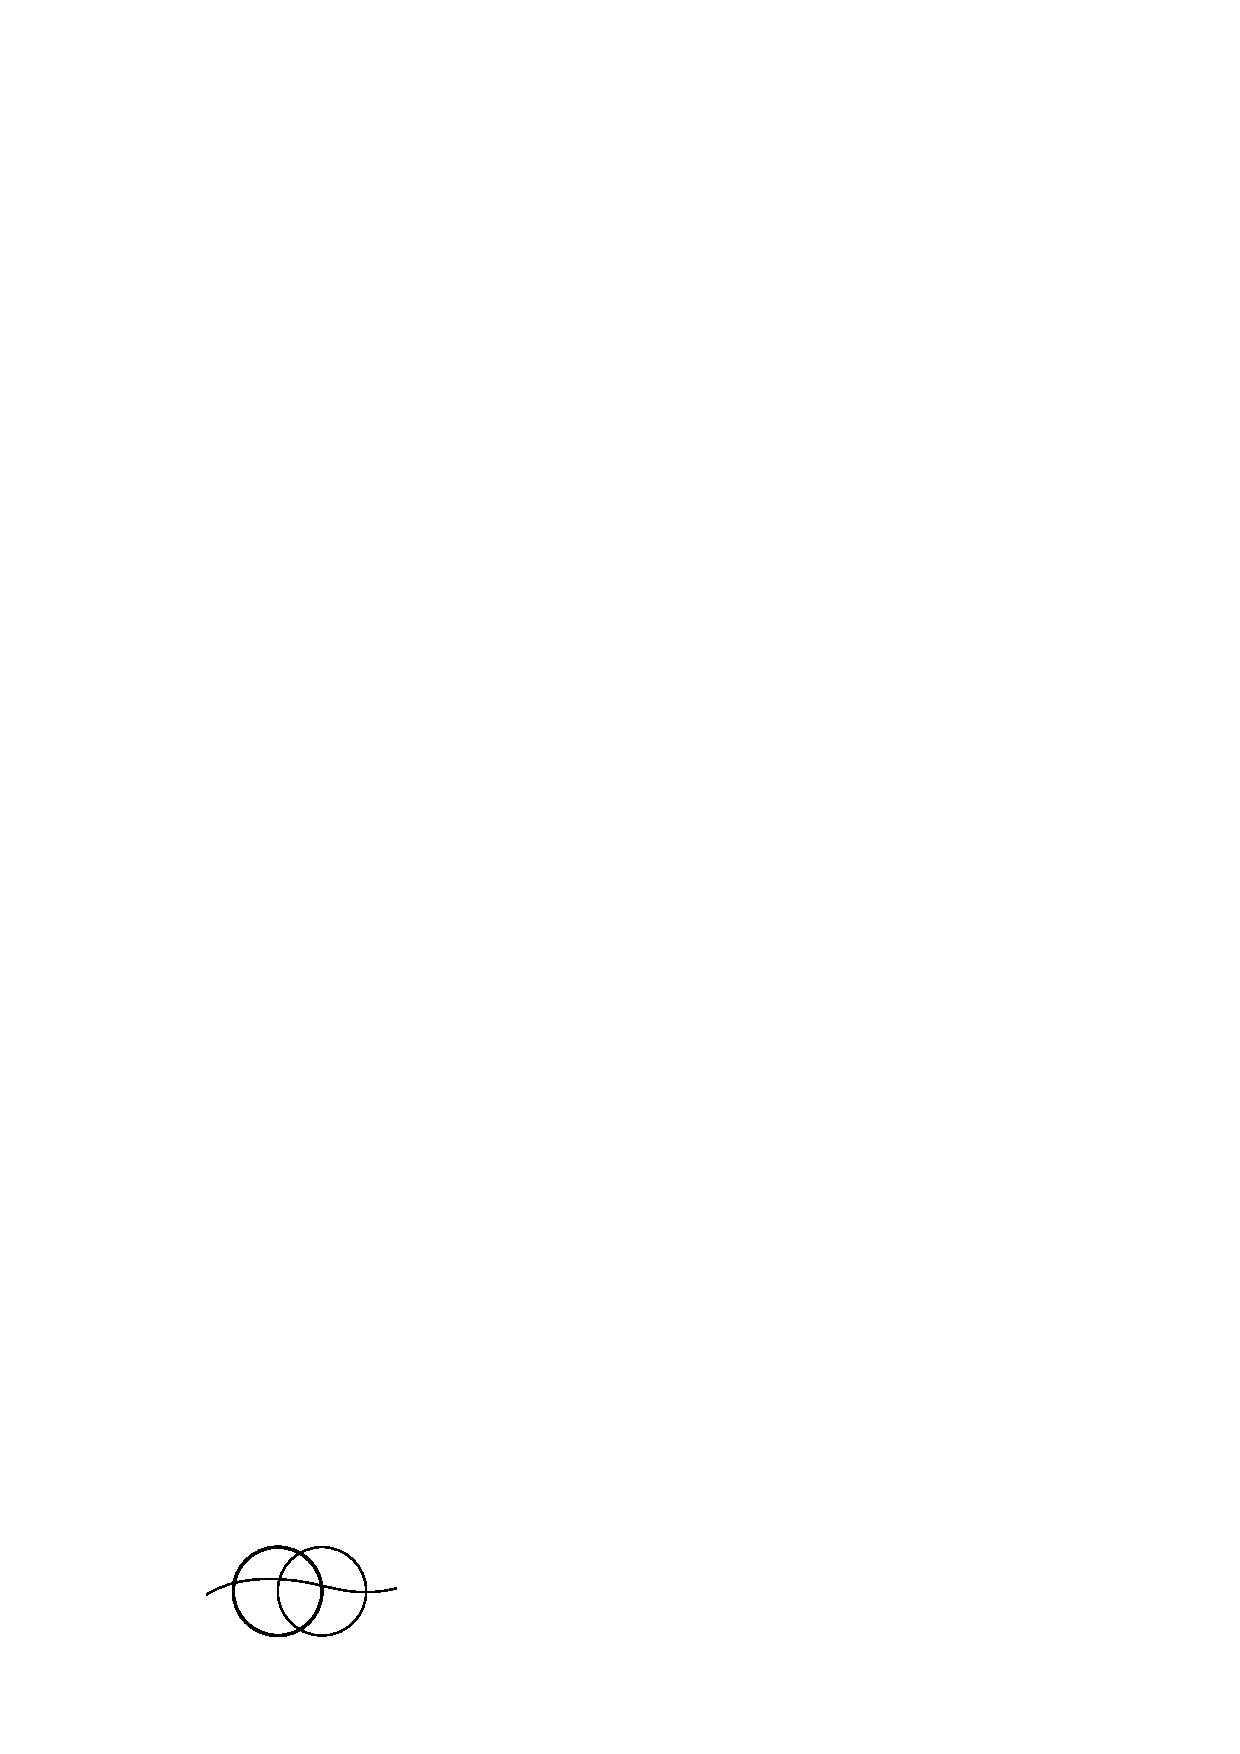
\includegraphics{graphics/mygraphic1.pdf}
  \else
    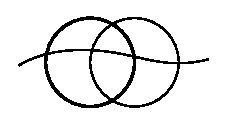
\includegraphics{graphics/mygraphic1-for-ps.eps}
  \fi
  \caption{Two circles and a wavy line.}
\end{figure}



\chapter{Conclusion and open questions}
\label{chap:conclusion}

This kind of chapter can include may different things (or only some of them):
\begin{itemize}
\item Discussion of results
\item Conclusions from the results or from the process in general
\item Open questions for future research, resulting from the research performed or from the results obtained
\end{itemize}

But not things like the bibliography or other back matter which is generated outside of this chapter.


\section{Some conclusion}

Here is what I conclude.

\section{Some open questions}

\paragraph{A question in brief.} In \autoref{chap:firstchap} we explored a certain subject, but what about this-or-that idea? Perhaps it is worth exploring. Can one produce interesting results?

\paragraph{A second question in brief.} A broader exposition of the question and indications of directions or ideas regarding its resolution.


%
% Add any appendices here; they must come _before_ the bibliography
%
\appendix
%\noappendicestocpagenum
%\addappheadtotoc

\chapter{Some sort of an appendix}
\label{appendix:somesort}

You may want to include appendices of your own volition. Also, if you've developed any computer software, that needs to go in as an appendix as well.

\section{A section}

Some appendix content here. And something nice to finish things off:

\begin{figure}[htb]
  \centering
  \ifpdf
    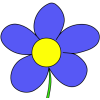
\includegraphics[width=0.3\textwidth]{graphics/mygraphic2.png}
  \else
    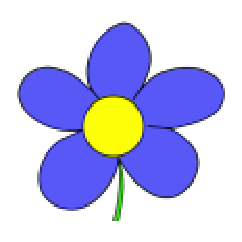
\includegraphics[width=0.3\textwidth]{graphics/mygraphic2-for-ps.eps}
  \fi
  \caption{A Flower.}
\end{figure}



% Back Matter
% ------------

% The following command will typeset the bibliography,
% then typeset the Hebrew part of the thesis:
% - Cover page
% - Title page
% - Acknowledgements page
%  (NO table of contents or list of figures in Hebrew)
% - (Extended) abstract (1000-2000 words)
%
% based on information you've provided in the thesis-fields file
% (including the relative paths to your bib files). The Hebrew
% content will be typeset in _reverse_page_order_, i.e. first
% in the file will be the last page of the abstract, and the
% Hebrew cover page will be the last page of the file.
%
\makebackmatter

% The resulting PDF can be printed and taken straight to binding,
% i.e. you do not need to flip any pages anywhere. Of course,
% mind the LaTeX error and warning messages, overfull hboxes etc.

\end{document}

